\section{Système embarqué}
\begin{frame}[t]
	\center{\huge{Système embarqué}}
	\begin{columns}
	\begin{column}[t]{0.30\linewidth}
		\begin{figure}
			\includegraphics<2->[height=2.5cm]{img/roomba.jpg}
			\uncover<2->{\caption{aspirateur du futur}}
		\end{figure}
	\end{column}
	\begin{column}[t]{0.30\linewidth}
		\begin{figure}
			\includegraphics<3->[height=2.5cm]{img/tesla.jpg}
			\uncover<3->{\caption{voiture du futur}}
		\end{figure}
	\end{column}
		\begin{column}[t]{0.30\linewidth}
		\begin{figure}
			\includegraphics<4->[height=2.5cm]{img/router.jpg}
			\uncover<4->{\caption{routeur normal}}
		\end{figure}
	\end{column}
	\end{columns}
	\uncover<5->{\center{Systèmes embarqués :)}}
\end{frame}

\begin{frame}[t]
	\center{\huge{Système embarqué}}
	\begin{columns}
	\begin{column}[t]{0.45\linewidth}
		\begin{figure}
			\includegraphics<2->[height=2.5cm]{img/raspi.jpg}
			\uncover<2->{\caption{Raspberry pi 2}}
		\end{figure}
	\end{column}
	\begin{column}[t]{0.45\linewidth}
		\begin{figure}
			\includegraphics<3->[height=2.5cm]{img/arduino.jpg}
			\uncover<3->{\caption{Arduino UNO}}
		\end{figure}
	\end{column}
	\end{columns}
	\uncover<4->{\center{Pas des systèmes embarqués :(}}
\end{frame}

% C'est quoi ?
\subsection{Contraintes}
\begin{frame}[t]
	\center{\huge{Contraintes}}
	\begin{block}<1->{Coûts matériels}
		\begin{itemize}
			\item Processeur
			\item Mémoire(s)
			\item Périphériques
		\end{itemize}
	\end{block}
	\begin{block}<2->{Coûts logiciels}
		\begin{itemize}
			\item Licenses ?
			\item Développements spécifiques ?
			\item Expertise ou support externe ?
			\item Evolution du produit ?
		\end{itemize}
	\end{block}
\end{frame}

\begin{frame}[t]
	\center{\huge{Contraintes}}
	\begin{block}{Performances}
		\begin{itemize}
			\item Latences : Temps réel
			\item Temps de boot
			\item Capacité de calcul
		\end{itemize}
	\end{block}
	\begin{block}<2->{Environnement}
		\begin{itemize}
			\item Durabilité
			\item Environnement physique hostile
			\item Consommation
			\item Normes ( Radio, GPS )
		\end{itemize}
	\end{block}
\end{frame}

\begin{frame}[t]
	\begin{block}<1->{Microcontrôleur}
		\begin{columns}[t]
			\begin{column}[T]{0.25\textwidth}
				\begin{figure}
					\includegraphics<1->[width=2.2cm]{img/atmega.jpg}
					\uncover<1->{\caption{Atmel ATMega 328}}
				\end{figure}
			\end{column}
			\begin{column}{0.70\textwidth}
				\begin{itemize}
					\item<2-> 1\euro50 / pièce
					\item<2-> 1 Cœur AVR 8bits @ 20 MHz
					\item<2-> 2 Ko RAM, 32 Ko Progmem
					\item<2-> I2C, SPI, UART
				\end{itemize}
			\end{column}
		\end{columns}
	\end{block}
	\begin{block}<3->{Microprocesseur}
		\begin{columns}[t]
			\begin{column}[T]{0.25\textwidth}
				\begin{figure}
					\includegraphics<3->[width=2.5cm]{img/imx.jpg}
					\uncover<3->{\caption{NXP iMX6 Quad}}
				\end{figure}
			\end{column}
			\begin{column}{0.70\textwidth}
				\begin{itemize}
					\item<4-> 36\euro / pièce
					\item<4-> 4 Cœurs ARM 32 bits @ 1GHz
					\item<4-> 256 Ko RAM, 96 Ko boot ROM
					\item<4-> DDR3, SDIO, eth, USB, HDMI, PCIe\dots
				\end{itemize}
			\end{column}
		\end{columns}
	\end{block}
\end{frame}


\begin{frame}
	\center{\huge{OS Temps-réel libres}}
	\begin{block}<2->{Contiki}
		\begin{columns}
		\begin{column}{0.50\textwidth}
		\begin{itemize}
			\item Orienté Networking et IoT
			\item Petite emprunte mémoire
			\item Riche en fonctionnalités
		\end{itemize}
		\end{column}
		\begin{column}{0.30\textwidth}
			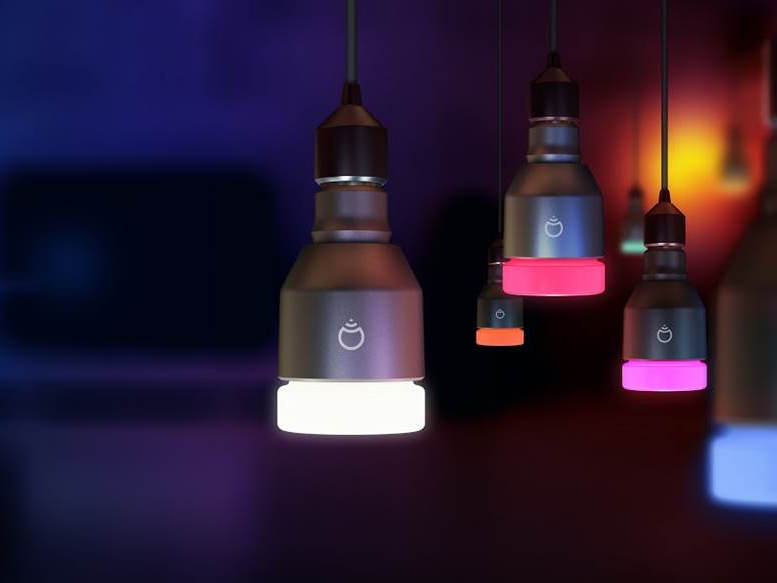
\includegraphics[height=2cm]{img/amp.jpg}
		\end{column}
		\end{columns}
	\end{block}
	\begin{block}<3->{freeRTOS}
		\begin{columns}
			\begin{column}{0.50\textwidth}
				\begin{itemize}
					\item Petite emprunte mémoire
					\item Beaucoup d'architectures
					\item Éprouvé dans l'industrie
				\end{itemize}
			\end{column}
			\begin{column}{0.20\textwidth}
				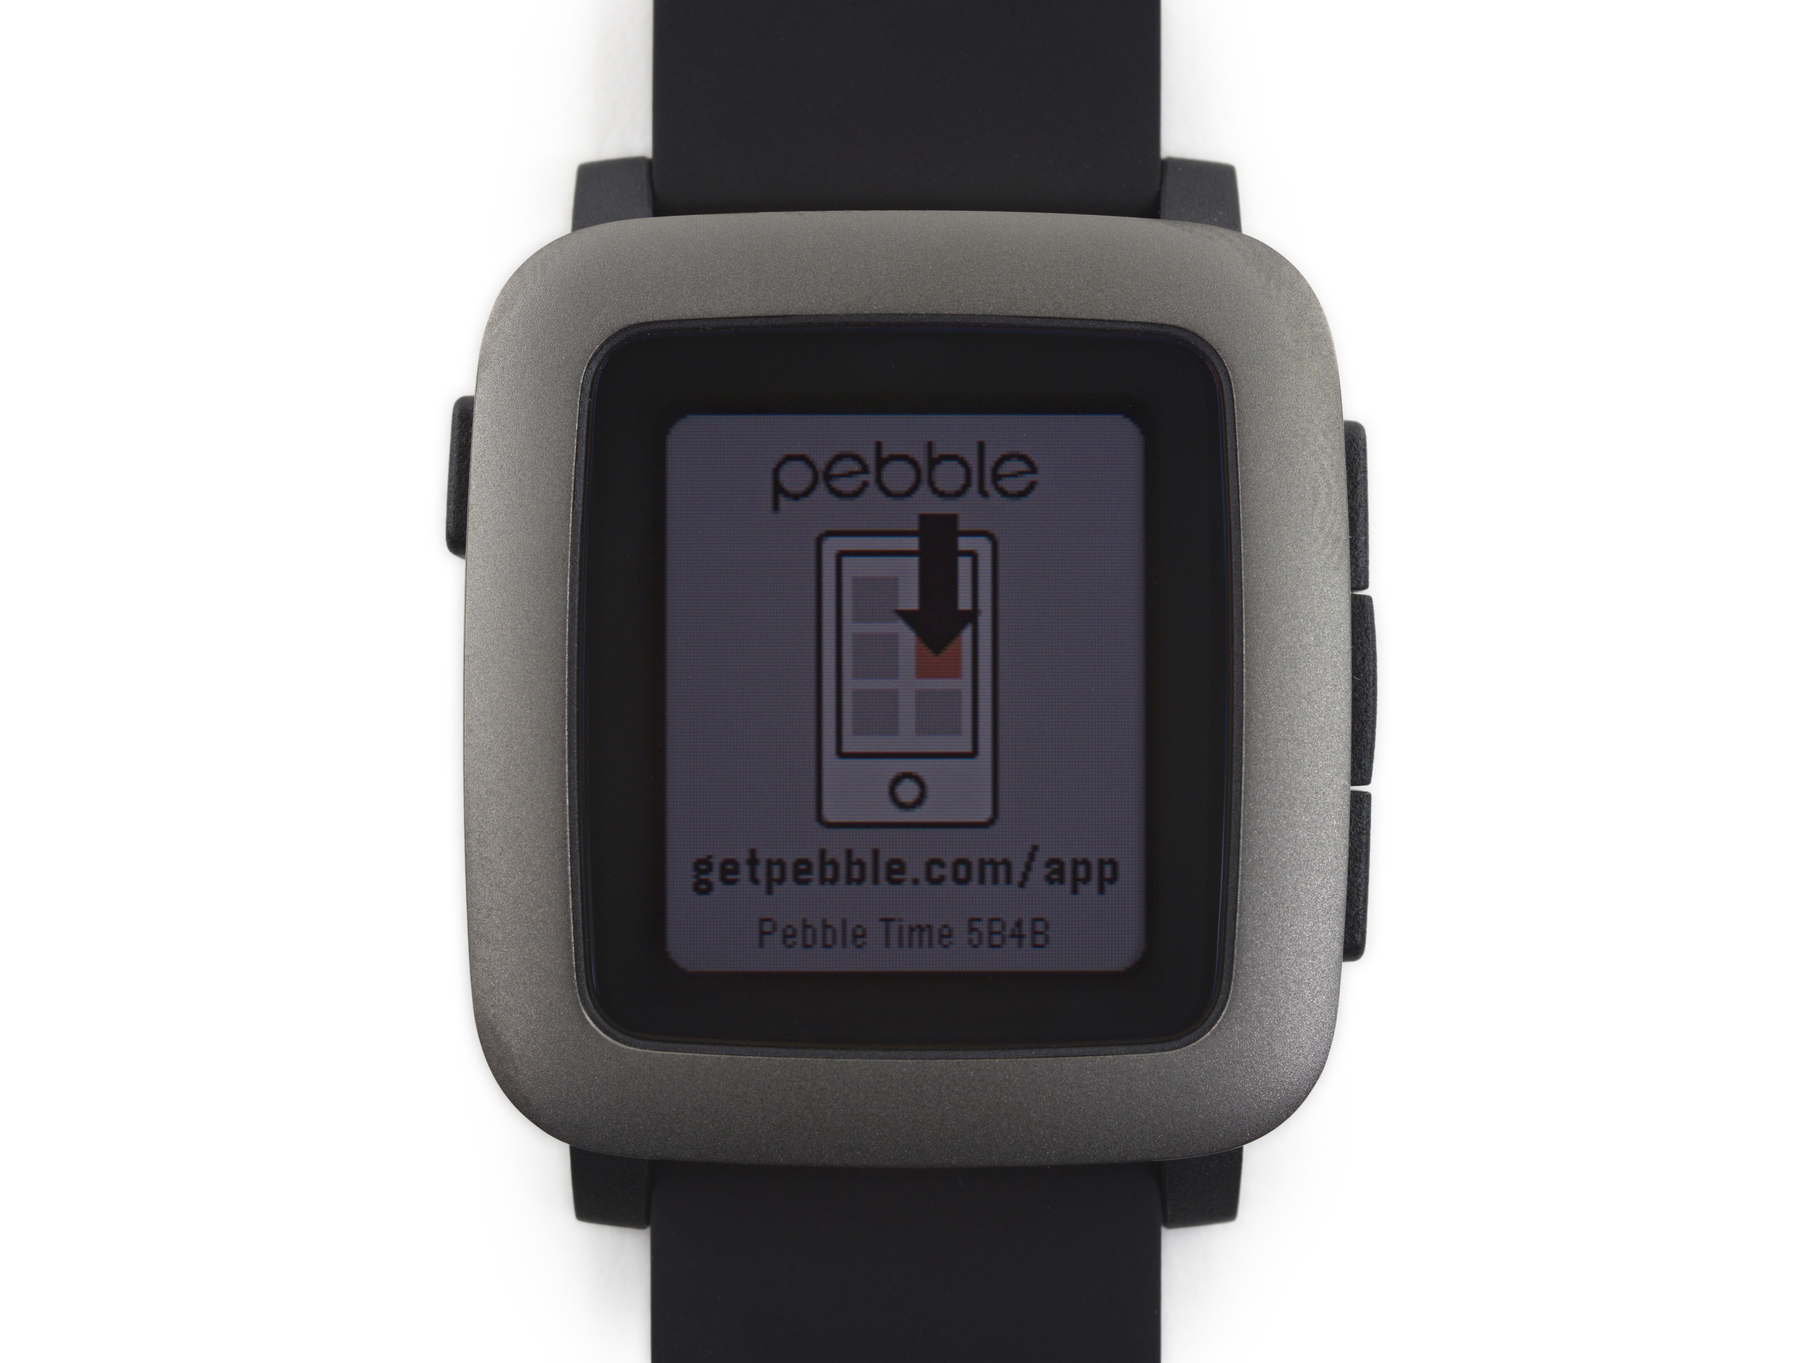
\includegraphics[height=2cm]{img/pt.jpg}
			\end{column}
			\begin{column}{0.20\textwidth}
				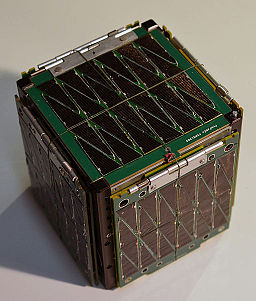
\includegraphics[height=2cm]{img/cubesat.jpg}
			\end{column}
		\end{columns}
	\end{block}
\end{frame}

